\documentclass[letter]{article}

%% Language and font encodings
\usepackage[english]{babel}
\usepackage[utf8x]{inputenc}
\usepackage[T1]{fontenc}
\usepackage{listings}
\usepackage{stmaryrd}
\usepackage{pgfplots}

%% Sets page size and margins
\usepackage[top=2cm,bottom=2cm,left=3cm,right=3cm,marginparwidth=1.75cm]{geometry}

%% Useful packages
\usepackage{amsmath}
\usepackage{amsfonts}
\usepackage{amssymb}
\usepackage{amsthm}
\usepackage{graphicx}
\usepackage[colorinlistoftodos]{todonotes}
%\usepackage[colorlinks=true, allcolors=blue]{hyperref}
\usepackage{array}
\usepackage[shortlabels]{enumitem}
\usepackage[final]{pdfpages}
\usepackage[normalem]{ulem}
\usepackage{cancel}
\usepackage{xspace,mdwlist}
\usepackage{algorithmic}
\usepackage{mathtools}
\usetikzlibrary{calc}

\usepackage{courier} %% Sets font for listing as Courier.
\usepackage{listings, xcolor}
\lstset{
tabsize = 4, %% set tab space width
showstringspaces = false, %% prevent space marking in strings, string is defined as the text that is generally printed directly to the console
numbers = left, %% display line numbers on the left
commentstyle = \color{green}, %% set comment color
keywordstyle = \color{blue}, %% set keyword color
stringstyle = \color{red}, %% set string color
rulecolor = \color{black}, %% set frame color to avoid being affected by text color
basicstyle = \small \ttfamily , %% set listing font and size
breaklines = true, %% enable line breaking
numberstyle = \tiny,
}



\DeclarePairedDelimiter{\ceil}{\lceil}{\rceil}
\DeclarePairedDelimiter{\floor}{\lfloor}{\rfloor}

\newtheorem{theorem}{Theorem}[section]
\newtheorem*{claim}{Claim}
\DeclareMathOperator*{\argmin}{\arg\!\min}

\def\coursename{CS 201: Data Structures}

%% make title box
\newcommand{\header}[1]{%
	\begin{center}
		\fbox{
			\begin{minipage}{6in}
				\textbf{\coursename} \hfill       \\
				\textit{#1} \hfill \textit{\today}
			\end{minipage}
		}
	\end{center}
	\vspace*{4mm}
}

\def\problem#1#2#3{
\fbox{
\begin{minipage}{0.8\textwidth}
{\sc #1:}

\begin{description*}
\item[Given:] #2
\item[Find:] #3
\end{description*}
\end{minipage}
}
\bigskip
}


\begin{document}

\header{Week 4: big-O, stacks, queues}

\begin{enumerate}[1.] 
    \item Big-O foundation
    \begin{itemize}
        \item [(a)] When evaluating the efficiency of a program, why do we use big-O notation instead of the \textit{performance}, which is the actual time to run the program?\\\\\\\\\\
        \item [(b)] In one sentence, what does big-O measure?\\\\\\\\\\
        \item [(c)] Provide the big-O notation and the names (constant, linear, quadratic, or logarithmic) for each function:\\\\

        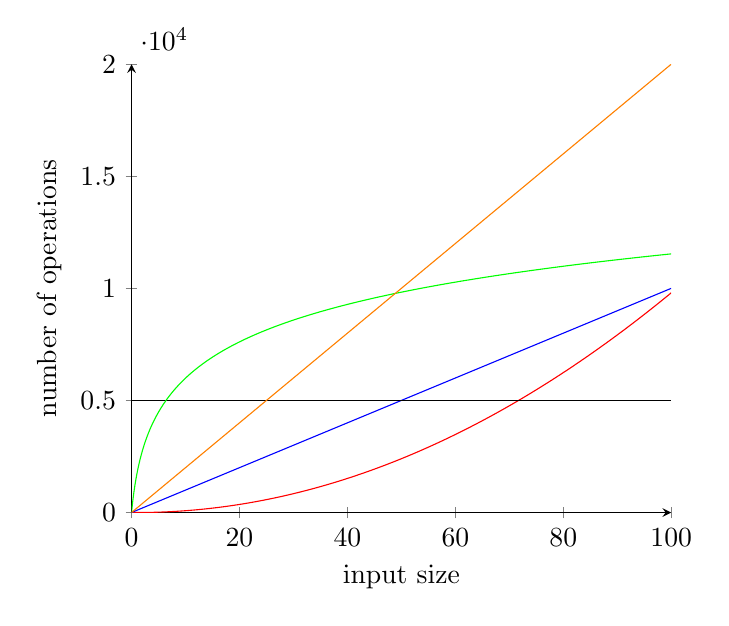
\begin{tikzpicture}
\begin{axis}[
    axis lines = left,
    xlabel = input size,
    ylabel = number of operations,
]
%Below the red parabola is defined
\addplot [
    domain=0:100, 
    samples=500, 
    color=red,
]
{x^2 - 2*x};
%Here the blue parabola is defined
\addplot [
    domain=0:100, 
    samples=500, 
    color=blue,
    ]
    {100*x};
\addplot [
    domain=0:100, 
    samples=500, 
    color=black,
    ]
    {5000};
\addplot [
    domain=0:100, 
    samples=500, 
    color=green,
    ]
    {ln(x+1)* 2500};
\addplot [
    domain=0:100, 
    samples=500, 
    color=orange,
    ]
    {200*x};
\end{axis}
\end{tikzpicture}

    \item [(d)] Arrange the functions in (c) in terms of how fast it grows as the input size increases to infinity.

    \end{itemize}

    \newpage
    \item Big-O Practice
    \begin{itemize}
    \item [(a)] What is the runtime complexity of the following LinkedList method?

    \begin{lstlisting}[language = Java , frame = trBL , firstnumber = 0 , escapeinside={(*@}{@*)}]
public int potato(int numItems) {
    int someNum = 0;
    Node<E> temp = head;
    while (temp != null) {
        if ((temp.data).equals(item)) { //You can assume that equals() is O(1)
            break;
        }
        temp = temp.next;
        someNum++;
    }
    if (count >= numItems) {
        return -1;
    }
    return someNum;
}
    \end{lstlisting}

    \item [(b)] What is the runtime complexity of the following LinkedList method?

    \begin{lstlisting}[language = Java , frame = trBL , firstnumber = 0 , escapeinside={(*@}{@*)}]
public boolean strawberry(Node<E> node) {
    if (node.next != null) {
        return true;
    }
    return false;
}
    \end{lstlisting}

    \item [(c)] What is the runtime complexity of the following method? (This one is challenging, so feel free to ask for hints!)

    \begin{lstlisting}[language = Java , frame = trBL , firstnumber = 0 , escapeinside={(*@}{@*)}]
public Integer[] whatIsThis(int numItems) {
    Integer[] numArray = new Integer[numItems];
    for (int i=0; i < numItems; i++) {
        int sum = 0;
        for (int j = i; j < numItems; j++) {
            sum += j;
        }
        numArray[i] = sum;
    }
    return numArray;
}
    \end{lstlisting}
    \end{itemize}
\newpage
    \item Stacks and Queues foundation
    \begin{itemize}
        \item [(a)] True/False: Stack is a LIFO (last in first out) ADT, while queue is a FIFO (first in first out) ADT.
        \item [(b)] (Adapted from Koffman-Wolfgang) What is the output of the following:

    \begin{lstlisting}[language = Java , frame = trBL , firstnumber = 0 , escapeinside={(*@}{@*)}]
Stack<String> myStack = new Stack<String>();
myStack.push("meow");
myStack.push("woof");
myStack.push("moo");
myStack.push("oink");
String sound = myStack.peek();

while (!myStack.isEmpty()) { //isEmpty returns true if stack is empty
    System.out.println(names.pop());
}
System.out.println(sound);
    \end{lstlisting}
    \item [(c)] (Adapted from Koffman-Wolfgang) What is the output of the following:

    \begin{lstlisting}[language = Java , frame = trBL , firstnumber = 0 , escapeinside={(*@}{@*)}]
Queue<String> myQueue = new Queue<String>();
myQueue.enqueue("meow");
myQueue.enqueue("woof");
myQueue.enqueue("moo");
myQueue.enqueue("oink");
String sound = myStack.peek();

while (!myStack.isEmpty()) { //isEmpty returns true if stack is empty
    System.out.println(names.dequeue());
}
System.out.println(sound);
    \end{lstlisting}
    \end{itemize}
    
    \item Dynamic array vs linked lists
    \begin{itemize}
        \item [(a)] What are the advantages and disadvantages of using a dynamic array vs linked list for a stack implementation?\\\\\\\\\\
        \item [(b)] What are the advantages and disadvantages of using a dynamic array vs linked list for a queue implementation?\\\\\\\\\\
    \end{itemize}

    \newpage
    \item (Adapted from Koffman-Wolfgang) A palindrome is a string which reads the same in either direction: left to right or right to left. For example, "kayak", "racecar" are palindromes. Write a method \textbf{public static boolean isPalindrome(String word)} that returns true if \textbf{word} is a palindrome, and false otherwise. You must use a stack in this method. 

    \begin{lstlisting}[language = Java , frame = trBL , firstnumber = 0 , escapeinside={(*@}{@*)}]
public static boolean isPalindrome(String word) {
    Stack<.........> myStack = ... Stack<........>();
    //Your code here
















}
    \end{lstlisting}
    
    \newpage
    \item Suppose we have an ArrayList implementation of a queue, myQueue, and its data array is ["c","a","b"], with front = 1, and rear = 0. 
    \begin{itemize}
        \item [(a)] Suppose I perform enqueue("d") on myQueue. Draw newArray and indicate the value of i for each iteration of the for loop.\\
        
        1st iteration: i = \\
        diagram of newArray:\\

        2nd iteration: i = \\
        diagram of newArray:\\

        3rd iteration: i = \\
        diagram of newArray:\\
        
        \item [(b)] After each method execution, what is the value of rear for myQueue?
            \begin{itemize}
                \item myQueue.enqueue("d"); 
                \item myQueue.enqueue("e"); 
                \item myQueue.enqueue("f"); 
            \end{itemize}
        
    \end{itemize} 

    \begin{lstlisting}[language = Java , frame = trBL , firstnumber = 0 , escapeinside={(*@}{@*)}]
public class Queue<E> {
    int numItems;
    int capacity; //the total number of slots in dataArray
    E[] dataArray;
    int front; //Index of the oldest item in the queue
    int rear; //Index of the most recent item in the queue
    public void enqueue(E item) {
        //expand the array if it is full
        if (numItems == capacity) {
            newArray = (E[]) new Object[capacity*2];
            for (int i = front; i < front + numItems; i++) {
                newArray[i] = data[i%capacity];
            }
            dataArray = newArray;
            rear = front + numItems; //adjust rear to its correct number
            capacity *= 2; //update the array capacity
        }
        //If we don't have to expand the array, then rear is gonna be a bit different
        else {
            rear = (rear + 1) % capacity;
        }
        data[rearIndex] = item; //finally, add the new item at index rear
    }
}

    \end{lstlisting}
\end{enumerate}
\end{document}
